%GNUPLOT: LaTeX picture with Postscript
\begin{picture}(0,0)%
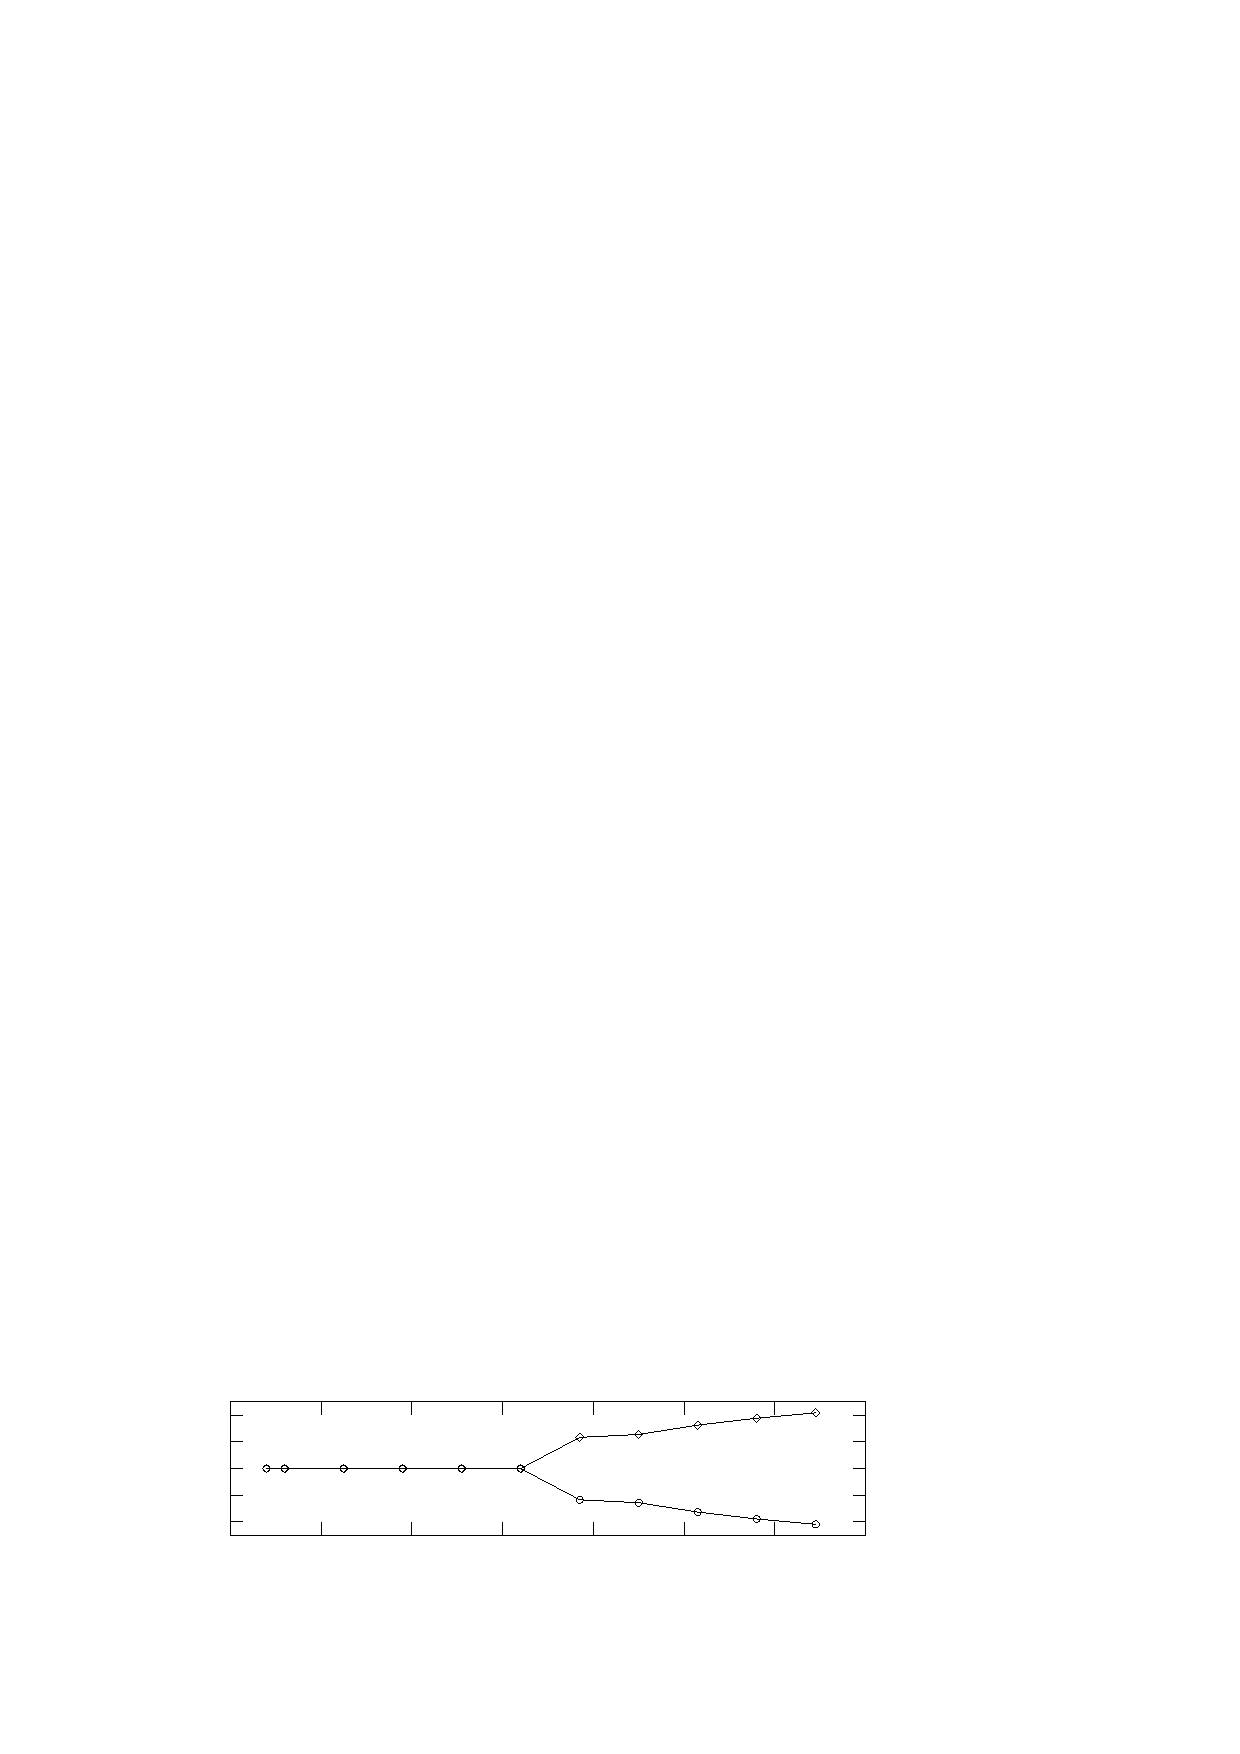
\includegraphics{bifurcacion-rounded}%
\end{picture}%
\begingroup
\setlength{\unitlength}{0.0200bp}%
\begin{picture}(18000,5400)(0,0)%
\put(1650,1970){\makebox(0,0)[r]{\strut{}-2}}%
\put(1650,2610){\makebox(0,0)[r]{\strut{}-1}}%
\put(1650,3250){\makebox(0,0)[r]{\strut{}0}}%
\put(1650,3890){\makebox(0,0)[r]{\strut{}1}}%
\put(1650,4530){\makebox(0,0)[r]{\strut{}2}}%
\put(1925,1100){\makebox(0,0){\strut{}0.000}}%
\put(4104,1100){\makebox(0,0){\strut{}0.001}}%
\put(6282,1100){\makebox(0,0){\strut{}0.002}}%
\put(8461,1100){\makebox(0,0){\strut{}0.003}}%
\put(10639,1100){\makebox(0,0){\strut{}0.004}}%
\put(12818,1100){\makebox(0,0){\strut{}0.005}}%
\put(14996,1100){\makebox(0,0){\strut{}0.006}}%
\put(17175,1100){\makebox(0,0){\strut{}0.007}}%
\put(550,3250){\rotatebox{90}{\makebox(0,0){\strut{}$x^\ast$}}}%
\put(9550,275){\makebox(0,0){\strut{}$P_o^\ast$}}%
\end{picture}%
\endgroup
\endinput
